%% =====================================================================
%%  4CroCEE 2027 -- full paper template (LaTeX)
%%
%%  Files: Definitions/CroCEE.cls (class), Definitions/Elsevier.bst
%%         (BibTeX style), Bibliography/references.bib, Figures/ (logo, figures)
%%  Compile: pdfLaTeX (or XeLaTeX/LuaLaTeX) + BibTeX + pdfLaTeX x2;
%%           Overleaf does this automatically.
%%
%%  Class options: fullpaper (default) | extended   -- see 4CroCEE_ExtendedAbstract.tex
%%                 noparindent, hyphenation, nourlunderline
%%  Commands:  \author[1]{Name}  \affiliation[1]{...}  \keywords{...}
%%             \figref{..} -> Fig. 1   \tabref{..} -> Table 1
%%             \Eqref{..} -> Eq. (1)   \vect{u}, \matr{K} -> bold symbols
%%             \tablenotes{..} -> explanations below a table
%%             \cite{a,b} -> [1,2]     \cite{a,b,c,d} -> [1--4]
%%  Editorial (filled in by the editors, leave empty):
%%             \paperdoi{10.xxxx/yyyy}   \firstpage{123}
%%  Template: Marin Grubišić and Vedran Jagodnik, with the assistance of Claude.
%% =====================================================================
\documentclass{Definitions/CroCEE}

\title{Title of the paper (printed in capitals automatically, max. two lines)}

\author[1]{First Author}
\author[2]{Second Author}
\author{… (first and last name of each author, separated by commas)}

\affiliation[1]{Position, affiliation, e-mail address}
\affiliation[2]{Position, affiliation, e-mail address}

%% Editorial information -- do not fill in; added by the editors
%\paperdoi{10.5592/CO/4CroCEE.2027.001}
%\firstpage{1}

\begin{document}

\maketitle

\begin{abstract}
The abstract needs to be the same as the one given in the accepted version. Adjustments are allowed only if they are necessary to take into account the suggestions of the reviewers. The abstract should summarize the context, content, and conclusions of the paper in 250 to 300 words. It should not indicate how the paper is organized. It should not be a table of contents in prose or an introduction. It should not contain references or equations. \textbf{The abstract is typeset automatically by the \texttt{abstract} environment (10\,pt Palatino, line spacing exactly 12\,pt); do not change the font size or spacing.}
\end{abstract}

\keywords{keywords1, keywords2, etc. Authors should suggest about 4--8 keywords for indexing purposes (separated by commas). Keywords are typeset automatically in italics, 10\,pt, by the \texttt{\textbackslash keywords} command.}

\section{General Appearance}

This document explains and illustrates how to prepare papers for the 4\textsuperscript{th} Croatian Conference on Earthquake Engineering -- 4CroCEE 2027 using the LaTeX template. Papers should not exceed \textbf{12 pages in length,} including the abstract, figures, tables, endnotes, and references. \textbf{The minimum number of pages is 6 and the maximum is 12}. Manuscripts must be written in English. Authors using LaTeX must submit the complete source files \textbf{(.tex, .bib and figure files)} together with the compiled PDF, and should ensure that the formatting complies with the guidelines below before submission. Note that the compilation of this example prints the warning that the paper has fewer than 6 pages; the warning disappears when the paper reaches the required length.

\section{Organization}

Following the abstract, it is recommended to begin with an Introduction section and end with a Conclusion section summarizing the main findings of the paper. All sections should be written and arranged in a concise and easy to follow style. \textbf{The page layout, the 11\,pt Palatino font, the line spacing (exactly 1.2 times the font size), the single-column text and the 1\,cm indentation of the second and the following paragraphs are set by the class file \texttt{CroCEE.cls}. Do not change the margins, font sizes or spacing, and do not modify the class file.} The template can be compiled with pdfLaTeX, XeLaTeX or LuaLaTeX; the bibliography is generated with BibTeX (see the References section).

Section headings are created with the \texttt{\textbackslash section} command and are typeset in bold, 13\,pt, as shown above. Subsection headings (\texttt{\textbackslash subsection}) are typeset in bold, 11\,pt. Use the starred forms (e.g., \texttt{\textbackslash section*}) for unnumbered headings such as Acknowledgements. The title is converted to capital letters automatically; text that must keep its case (e.g., units) is protected with \texttt{\textbackslash NoCaseChange\{kN\}}. Page numbers are not printed; they are added by the editors.

All tables, figures and equations used in the text are numbered automatically in sequence. Always refer to them using labels and the commands \texttt{\textbackslash tabref}, \texttt{\textbackslash figref} and \texttt{\textbackslash Eqref} instead of typing the numbers by hand, so that the numbering stays correct when the order changes. Please pay attention to the quality of the figures.

\subsection{Numbering of subsections}

Use the decimal system for headings with no more than three levels (\texttt{\textbackslash section}, \texttt{\textbackslash subsection}, \texttt{\textbackslash subsubsection}); the numbers are generated automatically.

\subsection{Tables and Figures}

Tables are referred to in the text as \tabref{tab:modes}, \texttt{\textbackslash tabref\{tab:modes\}} (giving ``Table 1'', ``Table 2'', etc.) and must be included as part of the text, as shown below. The caption of each table is placed \underline{above} the table and is centred, in 10\,pt font; with the template it is enough to put the \texttt{\textbackslash caption} command before the table body. Table content is set in 10\,pt font by default (not smaller than 8\,pt).

Tables should be formatted with the \texttt{booktabs} rules (\texttt{\textbackslash toprule}, \texttt{\textbackslash midrule} and \texttt{\textbackslash bottomrule}) and without vertical lines, double lines, shading or colour. The table should span the full text width: use the \texttt{tabularx} environment with the width \texttt{\textbackslash fulllength}, the centred stretching column type \texttt{C} and the standard centred column type \texttt{c}, as in \tabref{tab:modes}. Explanations of symbols and abbreviations are given below the table with the \texttt{\textbackslash tablenotes} command (9\,pt). A particularly wide table may protrude into the left margin by setting, e.g., \texttt{\textbackslash setlength\{\textbackslash extralength\}\{1cm\}} before the table; the table width \texttt{\textbackslash fulllength} then becomes the text width plus 1\,cm, and the \texttt{adjustwidth} environment inside the table shifts it by the same amount. Reset the value with \texttt{\textbackslash setlength\{\textbackslash extralength\}\{0cm\}} after the table.

\begin{table}
  \begin{adjustwidth}{-\extralength}{0cm}
  \caption{Dynamic properties of model.}
  \label{tab:modes}
  \begin{tabularx}{\fulllength}{cCCCC}
    \toprule
    \textbf{Mode} & \textbf{T (s)} & \textbf{Mx} & \textbf{My} & \textbf{MRz} \\
    \midrule
    1 & 0.116 & 0     & 0.833 & 0     \\
    2 & 0.087 & 0.755 & 0     & 0.076 \\
    3 & 0.062 & 0.076 & 0     & 0.755 \\
    4 & 0.029 & 0     & 0.167 & 0     \\
    5 & 0.021 & 0.153 & 0     & 0.016 \\
    6 & 0.015 & 0.016 & 0     & 0.154 \\
    \bottomrule
  \end{tabularx}

  \tablenotes{\textbf{Notes:} T---natural period of the mode; Mx, My, MRz---modal participation ratios in the x and y directions and for rotation about the vertical axis. Explanations of symbols and abbreviations are given here, below the table, in 9\,pt font.}
  \end{adjustwidth}
\end{table}

Figures are referred to in the text as \figref{fig:model}, \texttt{\textbackslash figref\{fig:model\}} (giving ``Fig. 1'', ``Fig. 2'', etc.) and must be included as part of the text. Colour figures can be used, with a minimum resolution of 300 dpi at the printed size; vector graphics (PDF) are preferred for diagrams and plots. (The example figure is a low-resolution placeholder and is therefore printed at 8.5\,cm; replace it with your own figure.) The caption must be independent of the corresponding figure and placed \underline{below} the figure (put the \texttt{\textbackslash caption} command after \texttt{\textbackslash includegraphics}). Figures are centred with the \texttt{\textbackslash centering} command inside the \texttt{figure} environment, and their width should not exceed the text width (e.g., \texttt{width=\textbackslash textwidth}).

\begin{figure}
  \centering
  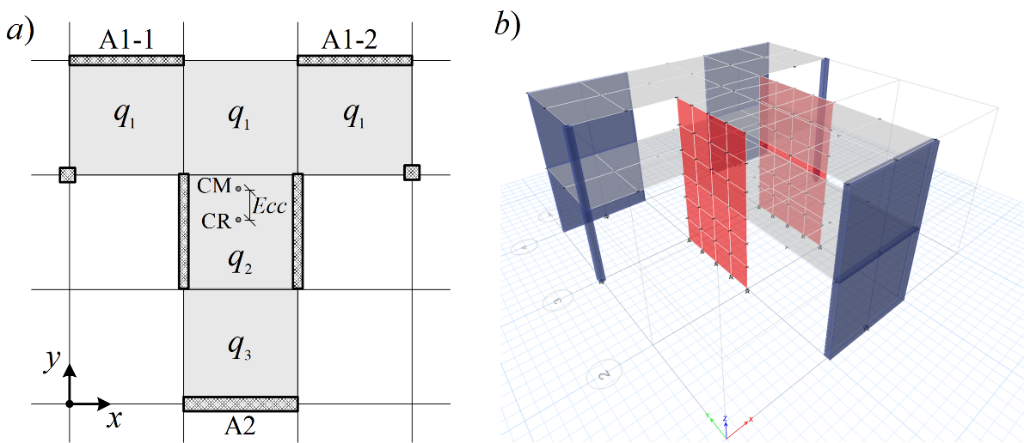
\includegraphics[width=12cm]{Figures/example_figure.png}
  \caption{a) Building plan; b) Numerical model.}
  \label{fig:model}
\end{figure}

\subsection{Lists, footnotes and endnotes}

Bulleted lists (\texttt{itemize}) and numbered lists (\texttt{enumerate}) are indented by 1.27\,cm:
\begin{itemize}
  \item first item;
  \item second item.
\end{itemize}

A footnote is created with \texttt{\textbackslash footnote}\footnote{Footnotes are set in 9\,pt font at the bottom of the page.}. Endnotes are created with \texttt{\textbackslash endnote}\endnote{Endnotes are collected in a list, which is printed where \texttt{\textbackslash printendnotes} is placed, usually before the References.} and printed with \texttt{\textbackslash printendnotes}. \paragraph{Run-in heading} A \texttt{\textbackslash paragraph} is a bold run-in heading without a number; it is not part of the Word template and should be used sparingly.

\section{Equations}

Symbols denoting vectors and matrices should be indicated in bold type; the commands \texttt{\textbackslash vect\{u\}} and \texttt{\textbackslash matr\{K\}} are provided for this purpose. Scalar variable names should normally be expressed using italics (the default in math mode), while units and descriptive subscripts are set upright (e.g., \texttt{\textbackslash mathrm\{max\}}). Weights and measures should be expressed in SI units, separated from the number by a thin space (e.g., \texttt{10\textbackslash,kN}). Equations are written in the \texttt{equation} environment (or \texttt{align} for several lines); they are centred on the page, and their numbers are right-aligned and placed in parentheses automatically. The equation font size and the 8\,pt of empty space above and below the equations are set by the class file. Equations are referred to in the body text in abbreviated form, e.g.,~\Eqref{eq:pythagoras} or \Eqref{eq:static}, using \texttt{\textbackslash Eqref\{label\}}, which produces ``Eq. (1)''. Displayed equations are numbered consecutively in the paper. Conventional symbols should be adopted and used consistently.

A simple equation is typeset as
\begin{equation}
  a^2 + b^2 = c^2
  \label{eq:pythagoras}
\end{equation}

An equation with a vector and a matrix, where $\matr{K}$ is the stiffness matrix, $\vect{u}$ the displacement vector and $\vect{f}$ the load vector, is typeset as
\begin{equation}
  \matr{K}\,\vect{u} = \vect{f}
  \label{eq:static}
\end{equation}

\section*{Acknowledgements}

Acknowledgements provide an opportunity to express appreciation to those who contributed significantly to the preparation of the paper. They may be written in free style and must be brief.

\section*{Copyrights}

4CroCEE 2027 reserves the copyright of the published proceedings. Authors will have the right to use the content of published papers, in part or in full, for their own work. Authors who use previously published data and illustrations must acknowledge the original source in the accompanying captions.

\printendnotes

%% (\setbibpreamble is optional text between the heading and the list;
%%  it is used here only to explain the style -- delete it in your paper)
\setbibpreamble{References must be cited in the text using square brackets, numbered according to the order in which they appear in the text, e.g. \cite{DAyala2003,Bommer2010} or \cite{Magenes2011,POLIMI2010,Kayen2014,Chopra2019,Brown2001,Trent1975,Kovac2020,Beyer2019,Horvat2019}, and listed at the end of the manuscript in a section called References. Citations are produced with \texttt{\textbackslash cite\{key\}}. The reference list follows the \emph{Elsevier (numeric, with titles)} style and is generated automatically by BibTeX from the file \texttt{Bibliography/References.bib} with the style \texttt{Definitions/Elsevier.bst}; only the cited works are listed, in order of first citation. The same style is available in Zotero and Mendeley under the same name, so that papers written in Word and in LaTeX use the same reference style. Examples of a journal article \cite{DAyala2003,Bommer2010}, a conference paper \cite{Magenes2011}, technical reports \cite{POLIMI2010,Kayen2014}, a book \cite{Chopra2019}, a book chapter \cite{Brown2001}, a doctoral and a master's thesis \cite{Trent1975,Kovac2020}, an electronic source \cite{Beyer2019} and a personal communication \cite{Horvat2019} are given below; the corresponding entries are in \texttt{Bibliography/References.bib}.}

\bibliographystyle{Definitions/Elsevier}
\bibliography{Bibliography/References}

\end{document}
